\documentclass[preview]{standalone}

\usepackage{amsmath}
\usepackage{amssymb}
\usepackage{stellar}
\usepackage{definitions}
\usepackage{blkarray}
\usepackage{tikz}

\begin{document}

\id{graphs}
\genpage

\section{Definitions}

\begin{snippetdefinition}{graph-definition}{Graph}
    A \textit{graph} is a tuple \((V,E)\) where
    \begin{itemize}
        \item \(V\) is a \set of \textit{vertices} or \textit{nodes};
        \item \(E \subseteq \{\{x,y\} \suchthat x,y \in V \land x \neq y\}\) is a set of \textit{edges}.
    \end{itemize}
\end{snippetdefinition}

\begin{snippetexample}{graph-example-1}{Example of a graph}
    Let \(G = (V, E)\) be a \graph where \(V = \{1, 2, 3, 4, 5, 6\}\) and
    \(E = \{\{1, 2\}, \{2, 3\}, \{3, 4\}, \{4, 5\}, \{5, 6\}\}\).
    \vspace{0.25cm}
    \begin{center}
			\tikzset{every picture/.style={line width=0.75pt}} %set default line width to 0.75pt        

			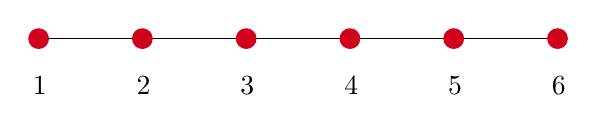
\begin{tikzpicture}[x=0.75pt,y=0.75pt,yscale=-1,xscale=1]
			%uncomment if require: \path (0,300); %set diagram left start at 0, and has height of 300

			%Straight Lines [id:da46250274214576614] 
			\draw    (175,115) -- (425,115) ;
			%Shape: Circle [id:dp08916666481415725] 
			\draw  [draw opacity=0][fill={rgb, 255:red, 208; green, 2; blue, 27 }  ,fill opacity=1 ] (220,115) .. controls (220,112.24) and (222.24,110) .. (225,110) .. controls (227.76,110) and (230,112.24) .. (230,115) .. controls (230,117.76) and (227.76,120) .. (225,120) .. controls (222.24,120) and (220,117.76) .. (220,115) -- cycle ;
			%Shape: Circle [id:dp7997596700799949] 
			\draw  [draw opacity=0][fill={rgb, 255:red, 208; green, 2; blue, 27 }  ,fill opacity=1 ] (270,115) .. controls (270,112.24) and (272.24,110) .. (275,110) .. controls (277.76,110) and (280,112.24) .. (280,115) .. controls (280,117.76) and (277.76,120) .. (275,120) .. controls (272.24,120) and (270,117.76) .. (270,115) -- cycle ;
			%Shape: Circle [id:dp04807433570988917] 
			\draw  [draw opacity=0][fill={rgb, 255:red, 208; green, 2; blue, 27 }  ,fill opacity=1 ] (320,115) .. controls (320,112.24) and (322.24,110) .. (325,110) .. controls (327.76,110) and (330,112.24) .. (330,115) .. controls (330,117.76) and (327.76,120) .. (325,120) .. controls (322.24,120) and (320,117.76) .. (320,115) -- cycle ;
			%Shape: Circle [id:dp6964194673091352] 
			\draw  [draw opacity=0][fill={rgb, 255:red, 208; green, 2; blue, 27 }  ,fill opacity=1 ] (370,115) .. controls (370,112.24) and (372.24,110) .. (375,110) .. controls (377.76,110) and (380,112.24) .. (380,115) .. controls (380,117.76) and (377.76,120) .. (375,120) .. controls (372.24,120) and (370,117.76) .. (370,115) -- cycle ;
			%Shape: Circle [id:dp5929377887646771] 
			\draw  [draw opacity=0][fill={rgb, 255:red, 208; green, 2; blue, 27 }  ,fill opacity=1 ] (420,115) .. controls (420,112.24) and (422.24,110) .. (425,110) .. controls (427.76,110) and (430,112.24) .. (430,115) .. controls (430,117.76) and (427.76,120) .. (425,120) .. controls (422.24,120) and (420,117.76) .. (420,115) -- cycle ;
			%Shape: Circle [id:dp5663003446831361] 
			\draw  [draw opacity=0][fill={rgb, 255:red, 208; green, 2; blue, 27 }  ,fill opacity=1 ] (170,115) .. controls (170,112.24) and (172.24,110) .. (175,110) .. controls (177.76,110) and (180,112.24) .. (180,115) .. controls (180,117.76) and (177.76,120) .. (175,120) .. controls (172.24,120) and (170,117.76) .. (170,115) -- cycle ;

			% Text Node
			\draw (171,132) node [anchor=north west][inner sep=0.75pt]    {$1$};
			% Text Node
			\draw (221,132) node [anchor=north west][inner sep=0.75pt]    {$2$};
			% Text Node
			\draw (271,132) node [anchor=north west][inner sep=0.75pt]    {$3$};
			% Text Node
			\draw (321,132) node [anchor=north west][inner sep=0.75pt]    {$4$};
			% Text Node
			\draw (371,132) node [anchor=north west][inner sep=0.75pt]    {$5$};
			% Text Node
			\draw (421,132) node [anchor=north west][inner sep=0.75pt]    {$6$};
			\end{tikzpicture}
	\end{center}
\end{snippetexample}

\begin{snippetdefinition}{graph-adjacent-vertices-definition}{Adjacent vertices}
    Let \(G=(V,E)\) be a \graph.
    Two vertices \(v_1,v_2 \in V\) are \textit{adjacent}
    if \(\{v_1,v_2\} \in E\).
\end{snippetdefinition}

\begin{snippetdefinition}{graph-adjacent-edges-definition}{Adjacent edges}
    Let \(G=(V,E)\) be a \graph.
    Two distinct edges \(e_1, e_2 \in E\) are \textit{adjacent}
    if \(e_1 \intersection e_2 \neq \emptyset \).
\end{snippetdefinition}

\begin{snippetdefinition}{graph-order-definition}{Order of a graph}
    Let \(G=(V,E)\) be a \graph.
    The \textit{order} of \(G\) is the number of vertices \(\cardinality{V}\).
\end{snippetdefinition}

\begin{snippetdefinition}{graph-size-definition}{Size of a graph}
    Let \(G=(V,E)\) be a \graph.
    The \textit{size} of \(G\) is the number of edges \(\cardinality{E}\).
\end{snippetdefinition}

\section{Adjacency Matrices}

\begin{snippetdefinition}{adjacency-matrix-definition}{Adjacency Matrix}
    A finite \graph can be represented by a square matrix
    \(n \times n\) where \(n\) is the number of vertices.

    \begin{center}
        \begin{minipage}[r]{6cm}
            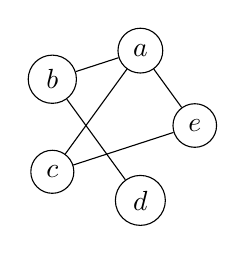
\begin{tikzpicture}[main/.style = {draw, circle}]
                \foreach \x [count = \xi] in {a,b,c,d,e} {
                    \node[main] (\xi) at
                        ({1 * cos(360 / 5 * \xi)}, {1 * sin(360 / 5 * \xi)})
                        {\(\x\)};
                }
            
                \draw (1) -- (2);
                \draw (1) -- (3);
                \draw (1) -- (5);
                \draw (2) -- (4);
                \draw (5) -- (3);
            \end{tikzpicture} 
        \end{minipage}
        \begin{minipage}[l]{6cm}
            A=
            \begin{blockarray}{cccccc}
                & a & b & c & d & e \\
                \begin{block}{c(ccccc)}
                a & 0 & 1 & 1 & 0 & 1 \\
                b & 1 & 0 & 0 & 1 & 0 \\
                c & 1 & 0 & 0 & 0 & 1 \\
                d & 0 & 1 & 0 & 0 & 0 \\
                e & 1 & 0 & 1 & 0 & 0 \\
                \end{block}
            \end{blockarray}
        \end{minipage}
    \end{center}

    Every row and column represents a vertex. \(1\) means
    that the two vertices are adjacent, \(0\) otherwise. The diagonal of this matrix
    will always e \(0s\) since no vertice is adjacent to itself
    and \(A=A^\transpose\)
\end{snippetdefinition}

\section{Degree}

\begin{snippetdefinition}{graph-vertex-degree-definition}{Degree}
    Let \(G=(V,E)\) be a \graph. The \textit{degree} of a vertex \(v \in V\), denoted \(\deg(v)\) is defined
    as the numbers of edges in \(E\) that are incident on \(v\).
\end{snippetdefinition}

\begin{snippetproposition}{graph-sum-of-degrees}{Sum of degrees of graph}
    Let \(G=(V,E)\) be a \graph.
    The sum of the \snippetref[graph-vertex-degree][degrees] of all vertices is equals to twice the number of edges.
    \[
        \sum_{v\in V}\graphdeg(v)=2|E|
    \]
\end{snippetproposition}

\section{Types of graphs}

\begin{snippetdefinition}{null-graph-definition}{Null graph}
    The \textit{null graph} is the \graph \((\emptyset, \emptyset)\).
\end{snippetdefinition}

\begin{snippetdefinition}{empty-graph-definition}{Empty graph}
    Let \(G=(V, E)\) be a \graph.
    \(G\) is an \textit{empty graph} if \(V = \emptyset\).
\end{snippetdefinition}

\begin{snippetdefinition}{trivial-graph-definition}{Trivial graph}
    Let \(G=(V, E)\) be a \graph.
    \(G\) is a \textit{trivial graph} if \(|V| = 1\).
\end{snippetdefinition}

\section{Subgraphs}

\begin{snippetdefinition}{improper-subgraph-definition}{Improper subgraph}
    Let \(G=(V_G, E_G)\) and \(H=(V_H,E_H)\) be \graph[graphs]. \\
    \(H\) is an \textit{improper subgraph} of \(G\), denoted \(H \subseteq G\),
    if \(V_H \subseteq V_G \land E_H \subseteq E_G\).
\end{snippetdefinition}

\begin{snippetdefinition}{proper-subgraph-definition}{Proper subgraph}
    Let \(G=(V_G, E_G)\) and \(H=(V_H,E_H)\) be \graph[graphs]. \\
    \(H\) is a \textit{proper subgraph} of \(G\), denoted \(H \subset G\),
    if \(V_H \subset V_G \land E_H \subset E_G\).
\end{snippetdefinition}

\begin{snippetdefinition}{spanning-subgraph-definition}{Spanning subgraph}
    Let \(G=(V_G, E_G)\) and \(H=(V_H,E_H)\) be \graph[graphs]. \\
    \(H\) is a \textit{spanning subgraph} of \(G\)
    if \(V_H = V_G \land E_H \subseteq E_G\).
\end{snippetdefinition}

\begin{snippetdefinition}{vertex-induced-subgraph-definition}{Vertex-Induced subgraph}
    Let \(G=(V, E)\) be a \graph and \(S \subseteq V\).
    The \textit{vertex-induced subgraph} of \(G\) by \(S\)
    is the subgraph of \(G\), denoted \(G[S]\), with vertices \(S\) and edges
    such that any two vertices \(v_1, v_2 \in G[S]\)
    are adjacent iff they are adjacent in \(G\).
    That is, \(G[S]\) has some vertices of \(G\) that are adjacent iff they are adjacent in \(G\).
\end{snippetdefinition}

\begin{snippetdefinition}{edge-induced-subgraph-definition}{Edge-Induced subgraph}
    Let \(G=(V, E)\) be a \graph and \(S \subseteq E\).
    The \textit{edge-induced subgraph} of \(G\) by \(S\)
    is the subgraph of \(G\), denoted \(G[S]\), with edges \(S\) and vertices
    such that for any vertex \(v \in G[S]\), \(v \subset e\)
    for some edge \(e \in S\).
    That is, \(G[S]\) has some edges of \(G\) and only vertices that are incident on said vertices.
\end{snippetdefinition}

\section{Paths}

\begin{snippetdefinition}{walk-definition}{Walk}
    Let \(G=(V, E)\) be a \graph.
    A \textit{walk} on \(G\) is a sequence of vertices in \(V\),
    where each consecutive pair of vertices are adjacent.
\end{snippetdefinition}

\begin{snippetdefinition}{trial-definition}{Trail}
    Let \(G=(V, E)\) be a \graph.
    A \textit{trail} on \(G\) is a sequence of vertices in \(V\),
    where each consecutive pair of vertices are adjacent but no edge can be traversed multiple times.
\end{snippetdefinition}

\begin{snippetdefinition}{path-definition}{Path}
    Let \(G=(V, E)\) be a \graph.
    A \textit{path} on \(G\) is a sequence of vertices in \(V\),
    where each consecutive pair of vertices are adjacent but no vertex can be traversed multiple times.
\end{snippetdefinition}

\begin{snippetdefinition}{ciclic-path-definition}{Cycle}
    Let \(P\) be a \path on \(G=(V, E)\).
    The path is said to be \textit{cycle} if it starts and end at the same vertex.
\end{snippetdefinition}

\begin{snippetdefinition}{simple-path-definition}{Simple path}
    Let \(P\) be a \path on \(G=(V, E)\).
    The path is said to be \textit{simple} if every vertex in it is distinct.
\end{snippetdefinition}

\begin{snippetdefinition}{connected-path-definition}{Connected path}
    Let \(G=(V, E)\) be a \graph.
    The graph is said to be \textit{connected} if there exist
    at least a \path between any pair of vertices.
\end{snippetdefinition}

\begin{snippetexample}{graph-connectivity-cn-example}{Connectivity of \(C_n\)}
	Consider the graph $C_n$ for $n \geq 3$.
	\begin{center}
		

\tikzset{every picture/.style={line width=0.75pt}} %set default line width to 0.75pt        

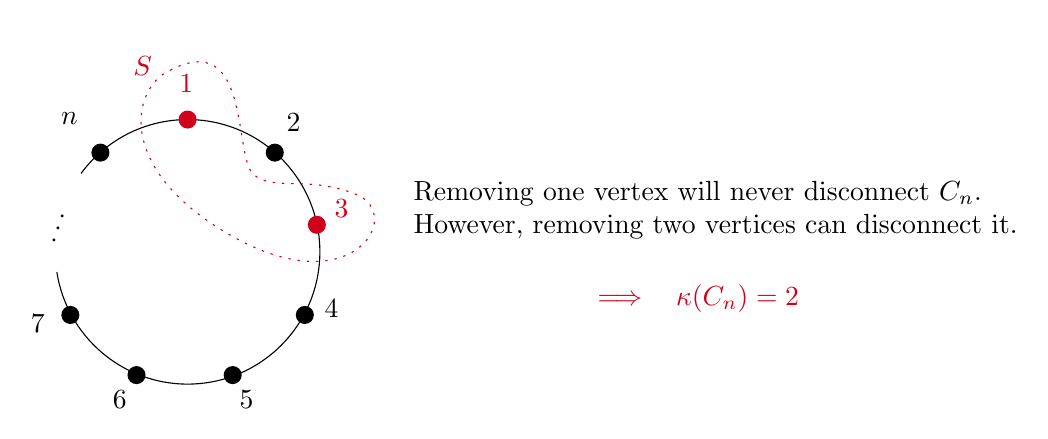
\begin{tikzpicture}[x=0.75pt,y=0.75pt,yscale=-1,xscale=1]
%uncomment if require: \path (0,244); %set diagram left start at 0, and has height of 244

%Shape: Arc [id:dp4708029626642417] 
\draw  [draw opacity=0] (147.09,79.71) .. controls (158.69,63.97) and (177.36,53.75) .. (198.42,53.75) .. controls (233.62,53.75) and (262.15,82.28) .. (262.15,117.48) .. controls (262.15,152.68) and (233.62,181.21) .. (198.42,181.21) .. controls (166.53,181.21) and (140.11,157.77) .. (135.43,127.19) -- (198.42,117.48) -- cycle ; \draw   (147.09,79.71) .. controls (158.69,63.97) and (177.36,53.75) .. (198.42,53.75) .. controls (233.62,53.75) and (262.15,82.28) .. (262.15,117.48) .. controls (262.15,152.68) and (233.62,181.21) .. (198.42,181.21) .. controls (166.53,181.21) and (140.11,157.77) .. (135.43,127.19) ;
%Shape: Ellipse [id:dp663608297444586] 
\draw  [draw opacity=0][fill={rgb, 255:red, 208; green, 2; blue, 27 }  ,fill opacity=1 ] (194.08,53.75) .. controls (194.08,51.35) and (196.02,49.41) .. (198.42,49.41) .. controls (200.82,49.41) and (202.77,51.35) .. (202.77,53.75) .. controls (202.77,56.15) and (200.82,58.1) .. (198.42,58.1) .. controls (196.02,58.1) and (194.08,56.15) .. (194.08,53.75) -- cycle ;
%Shape: Ellipse [id:dp6954182191954329] 
\draw  [draw opacity=0][fill={rgb, 255:red, 0; green, 0; blue, 0 }  ,fill opacity=1 ] (236.08,69.68) .. controls (236.08,67.28) and (238.03,65.34) .. (240.43,65.34) .. controls (242.83,65.34) and (244.77,67.28) .. (244.77,69.68) .. controls (244.77,72.08) and (242.83,74.03) .. (240.43,74.03) .. controls (238.03,74.03) and (236.08,72.08) .. (236.08,69.68) -- cycle ;
%Shape: Circle [id:dp9749161979355754] 
\draw  [draw opacity=0][fill={rgb, 255:red, 208; green, 2; blue, 27 }  ,fill opacity=1 ] (256.36,104.44) .. controls (256.36,102.04) and (258.3,100.1) .. (260.7,100.1) .. controls (263.1,100.1) and (265.05,102.04) .. (265.05,104.44) .. controls (265.05,106.84) and (263.1,108.79) .. (260.7,108.79) .. controls (258.3,108.79) and (256.36,106.84) .. (256.36,104.44) -- cycle ;
%Shape: Ellipse [id:dp42403131489300416] 
\draw  [draw opacity=0][fill={rgb, 255:red, 0; green, 0; blue, 0 }  ,fill opacity=1 ] (250.56,147.89) .. controls (250.56,145.5) and (252.51,143.55) .. (254.91,143.55) .. controls (257.31,143.55) and (259.25,145.5) .. (259.25,147.89) .. controls (259.25,150.29) and (257.31,152.24) .. (254.91,152.24) .. controls (252.51,152.24) and (250.56,150.29) .. (250.56,147.89) -- cycle ;
%Shape: Circle [id:dp735948108869646] 
\draw  [draw opacity=0][fill={rgb, 255:red, 0; green, 0; blue, 0 }  ,fill opacity=1 ] (215.8,176.86) .. controls (215.8,174.46) and (217.75,172.52) .. (220.15,172.52) .. controls (222.55,172.52) and (224.49,174.46) .. (224.49,176.86) .. controls (224.49,179.26) and (222.55,181.21) .. (220.15,181.21) .. controls (217.75,181.21) and (215.8,179.26) .. (215.8,176.86) -- cycle ;
%Shape: Circle [id:dp361614150375666] 
\draw  [draw opacity=0][fill={rgb, 255:red, 0; green, 0; blue, 0 }  ,fill opacity=1 ] (169.46,176.86) .. controls (169.46,174.46) and (171.4,172.52) .. (173.8,172.52) .. controls (176.2,172.52) and (178.15,174.46) .. (178.15,176.86) .. controls (178.15,179.26) and (176.2,181.21) .. (173.8,181.21) .. controls (171.4,181.21) and (169.46,179.26) .. (169.46,176.86) -- cycle ;
%Shape: Ellipse [id:dp799299292223014] 
\draw  [draw opacity=0][fill={rgb, 255:red, 0; green, 0; blue, 0 }  ,fill opacity=1 ] (137.59,147.89) .. controls (137.59,145.5) and (139.54,143.55) .. (141.94,143.55) .. controls (144.34,143.55) and (146.28,145.5) .. (146.28,147.89) .. controls (146.28,150.29) and (144.34,152.24) .. (141.94,152.24) .. controls (139.54,152.24) and (137.59,150.29) .. (137.59,147.89) -- cycle ;
%Shape: Rectangle [id:dp5189451174903476] 
\draw  [draw opacity=0][fill={rgb, 255:red, 255; green, 255; blue, 255 }  ,fill opacity=0 ] (123.11,76.93) -- (163.66,76.93) -- (163.66,123.27) -- (123.11,123.27) -- cycle ;
%Shape: Ellipse [id:dp2783474184800838] 
\draw  [draw opacity=0][fill={rgb, 255:red, 0; green, 0; blue, 0 }  ,fill opacity=1 ] (152.08,69.68) .. controls (152.08,67.28) and (154.02,65.34) .. (156.42,65.34) .. controls (158.82,65.34) and (160.77,67.28) .. (160.77,69.68) .. controls (160.77,72.08) and (158.82,74.03) .. (156.42,74.03) .. controls (154.02,74.03) and (152.08,72.08) .. (152.08,69.68) -- cycle ;
%Curve Lines [id:da09228568553946859] 
\draw [color={rgb, 255:red, 208; green, 2; blue, 27 }  ,draw opacity=1 ] [dash pattern={on 0.84pt off 2.51pt}]  (190,30) .. controls (229,9.75) and (220.5,71.25) .. (230,80) .. controls (239.5,88.75) and (257,80.25) .. (280,90) .. controls (303,99.75) and (278,142.75) .. (220,110) .. controls (162,77.25) and (172,37.75) .. (190,30) -- cycle ;

% Text Node
\draw (131.16,114.02) node [anchor=north west][inner sep=0.75pt]  [rotate=-289.59]  {$\dotsc $};
% Text Node
\draw (193.17,31) node [anchor=north west][inner sep=0.75pt]  [color={rgb, 255:red, 208; green, 2; blue, 27 }  ,opacity=1 ]  {$1$};
% Text Node
\draw (244.83,49.55) node [anchor=north west][inner sep=0.75pt]    {$2$};
% Text Node
\draw (268,91.1) node [anchor=north west][inner sep=0.75pt]  [color={rgb, 255:red, 208; green, 2; blue, 27 }  ,opacity=1 ]  {$3$};
% Text Node
\draw (263.21,139.45) node [anchor=north west][inner sep=0.75pt]    {$4$};
% Text Node
\draw (222.17,183) node [anchor=north west][inner sep=0.75pt]    {$5$};
% Text Node
\draw (161.2,183) node [anchor=north west][inner sep=0.75pt]    {$6$};
% Text Node
\draw (121.64,146.45) node [anchor=north west][inner sep=0.75pt]    {$7$};
% Text Node
\draw (136.17,49) node [anchor=north west][inner sep=0.75pt]    {$n$};
% Text Node
\draw (306,82) node [anchor=north west][inner sep=0.75pt]   [align=left] {Removing one vertex will never disconnect $\displaystyle C_{n}$.\\However, removing two vertices can disconnect it.};
% Text Node
\draw (391,132) node [anchor=north west][inner sep=0.75pt]  [color={rgb, 255:red, 208; green, 2; blue, 27 }  ,opacity=1 ]  {$\implies \ \ \kappa ( C_{n}) =2$};
% Text Node
\draw (171,22) node [anchor=north west][inner sep=0.75pt]  [color={rgb, 255:red, 208; green, 2; blue, 27 }  ,opacity=1 ]  {$S$};


\end{tikzpicture}
	\end{center}
\end{snippetexample}

\end{document}